\section{Cel dokumentu}
\suppressfloats[t]

Dokument ma na celu przedstawienie najważniejszych procesów w Systemie Obsługi Konferencji (SOK) w przejrzysty i czytelny sposób. Procesy zaprezetnowano z użyciem diagramów aktywności.

\section{Dokumenty i pliki powiązane}

\begin{itemize}
  \item \textit{Artykul.vsdx} - diagram aktywności procesu dodawania i recenzowania artykułu (plik programu Microsoft Visio 2013)
  \item \textit{Artykul.png} - wyeksportowany diagram aktywności cyklu życia artykułu
  \item \textit{DodawanieKonta.vsdx} - diagram aktywności procesu dodawania kont użytkowników do systemu (plik programu Microsoft Visio 2013)
  \item \textit{DodawanieKonta.png} - wyeksportowany diagram aktywności dodawania użytkowników
  \item \textit{Wycieczka.vsdx} - diagram aktywności przedstawiający cykl życia bytu Wycieczka w systemie (plik programu Microsoft Visio 2013)
  \item \textit{Wycieczka.png} - wyeksportowany diagram aktywności cyklu życia wycieczki 
\end{itemize}

\section{Procesy w systemie}

W każdym systemie możemy wyróżnić całą masę procesów które można opisać za pomocą diagramów aktywności, niektóre jednak są na tyle proste że nie wymagają komentarza w postaci diagramu. Dla zobrazowania ostatniego zdania opisowo przedstawię proces zmiany danych teleadresowych (telefon, e-mail)  użytkownika systemu. Zalogowany użytkownik wchodzi w zakładkę ``''Zarządzanie kontem'', klika w polu oznaczonym etykietą ``Numer telefonu'' wpisuje nowy numer telefonu i akceptuje klawiszem enter. To cały proces, jak widać nie ma tu nic specjalnego do opisywania każdy kto kiedykolwiek używał internetu poradzi sobie z takim procesem. Celem tego dokumentu jeest przedstawienie procesów które mogą okazać się nieoczywiste dla osób którym przypadnie implementacja i używanie systemu, wtedy można skorzystać z niniejszego dokumentu w celu sprawdzenia drogi przepływu informacji w danym procesie. Na tym etapie wyróżniliśmy trzy procesy które wydają się nie być oczywiste i mogą wymagać komentarza, jest to ``Definiowanie nowego użytkownika w systemie'' gdzie osobą która rejestruje jest ``bezpośredni przełożony'' nowego użytkownika czyli dla Pracownika będzie to Administrator, dla Rodziny Pracownika Pracownik. Administrator według wstępnych założeń jest jeden na cały system. Drugim wyróżnionym procesem jest dodawanie wycieczki, a ostatnim dodawanie i recenzowanie artykułu.

\section{Diagramy aktywności}

Żeby rozpocząć omawianie procesów za pomocą diagramów aktywności trzeba na początku krótko zcharakteryzować co tak na prawdę taki diagram przedstawia, a więc diagram akywności jest diagramem interakcji, który służy do modelowania dynamicznych aspektów systemu. Jego zasadniczą funkcją jest przedstawienie sekwencji kroków, które są wykonywane przez modelowany fragment systemu. Diagram sekwencji pozwala także na prezentację przepływów współbieżnych oraz na zaprezentowanie zmian stanów obiektów podczas przechodzenia pomiędzy czynnościami.  Definiując ogólnie, diagram aktywności jest stosowany do modelowania behawioralnych aspektów systemu i obrazuje strumień kolejno wykonywanych czynności, dlatego diagram aktywności nazywa się również diagramem czynności.

\subsection{Definiowanie nowego użytkownika w systemie}

\begin{figure}[!h]
    \centering
    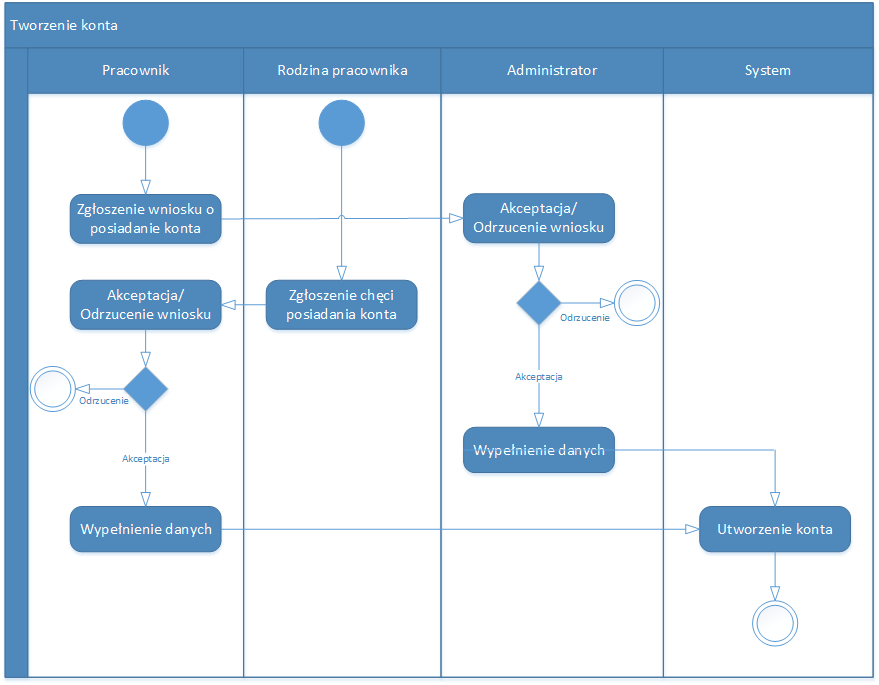
\includegraphics[width=\textwidth,height=4.7in]{DodawanieKonta.png}
    \caption{Model diagramu aktywności dodawania nowego konta do systemu.}
    \label{fig:dodawaniekonta}
\end{figure}

Jak widać proces może zostać zapoczątkowany przez pracownika jak i przez rodzinę pracownika, a pierwszym krokiem jest zgłoszenie chęci posiadania konta, może się to odbywać ``ustnie'' lub za pomocą na przykład wiadomości e-mail. Pracownik swoją prośbę przekazuje do Administratora systemu, natomiast Rodzina Pracownika do samego Pracownika, osoba ta może zaakceptować wniosek, wtedy wypełnia w systemie formularz z danymi przekazanymi mu we wniosku i tworzy w systemie nowe konto. Dla konta Pracownik Administrator musi wypełnić dodatkowo obligatoryjne pole specjalizacjia. Specjalizację definiować będą etykiety słownikowe, do pracownika trzeba będzie przyporządkować co najmniej jedną etykietę.

\subsection{Cykl życia wycieczki w systemie}

\begin{figure}[!tb]
    \centering
    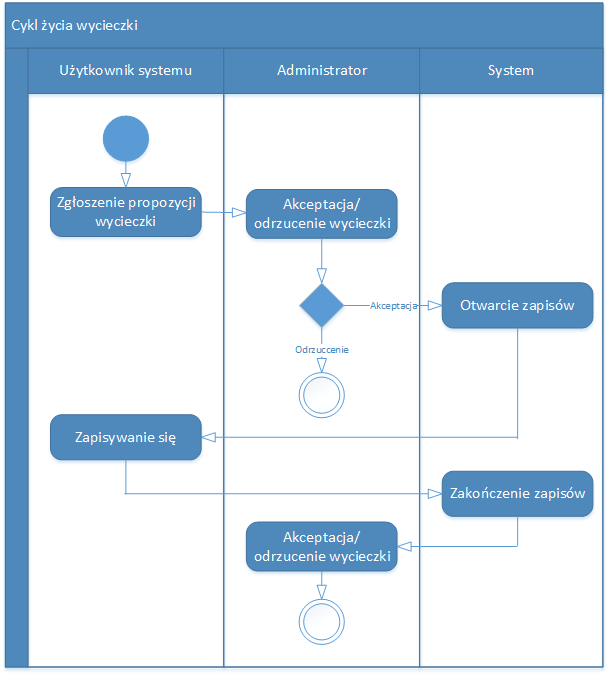
\includegraphics[width=\textwidth,height=5in]{Wycieczka.png}
    \caption{Model diagramu aktywności bytu wycieczka w systemie.}
    \label{fig:wycieczka}
\end{figure}

Zgłosić propozycję wycieczki w systemie może każdy, wypełnia wtedy odpowiedni formularz zgłoszeniowy. Formularz trafia do akceptacji przez Administratora Systemu i ten decyduje czy przyjąć wniosek, jeżeli tak zrobi projekt wycieczki staje się dostępny dla wszystkich użytkowników i otwierają się zapisy. administrator jednocześnie ustala termin zapisów, po upłynięciu tego czasu Administrator decyduje czy wycieczka się odbędzie czy też nie (na przykład zbyt mało chętnych) i ustawia odpowiedni status wycieczki, pojawia się odpowiednia infromacja w panelu Aktualności.

\subsection{Przepływ artykułów w systemie}

\begin{figure}[!tb]
    \centering
    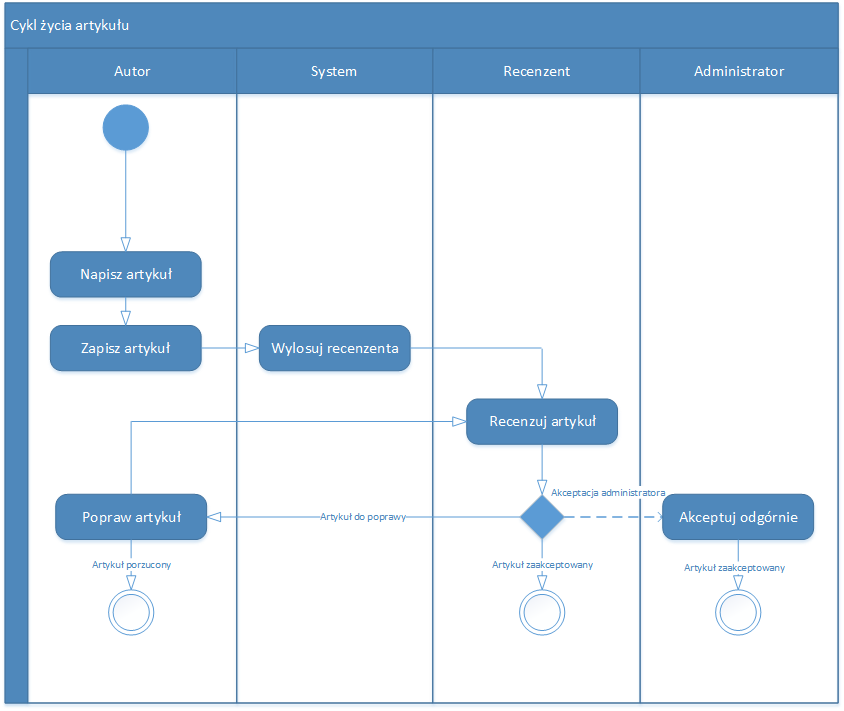
\includegraphics[width=\textwidth,height=5in]{Artykul.png}
    \caption{Model diagramu aktywności przepyłwu artykułów w systemie.}
    \label{fig:rodzina}
\end{figure}


Proces zaczyna się od zgłoszenia przez Pracownika systemu ``Autora'' tematu artykułu oraz dodanie do niego etykiet ze słownika systemowego które definiowały będą do jakiej kategorii ów temat się zalicza (na przykład mikrokontrolery, technika wysokich napięć, maszyny elektryczne itp.) można przypisać kilka etykiet do artykułu, ale musi być co najmniej jedna, jeżeli temat zostanie zaakceptowany przez Administratora autor zaczyna pracę, jeżeli uzna że już skończył wysyła artykuł do systemu który spośród innych Pracowników którzy również posiadają etykiety z tego samego słownika  (na przykład mikrokontrolery, technika wysokich napięć, maszyny elektryczne itp.)  przydziela mu według specjalnego algorytmu najlepszego przyporządkowania, osobę która najlepiej pasuje do etykiet przyporządkowanych do artykułu, Autor' nie zna swojego recenzenta i vice versa. Teraz jeżeli recenzent uzna że aktykuł trzeba poprawić wysyła go spowrotem do autora który poprawia wszystkie zgłoszone przez recenzenta uwagi i wysyła ponownie do recenzenta i tak w kłko dopóki recenzent nie zaakceptuje artykułu lub autor go nie porzuci.

\section{Historia Zmian}

\begin{tabularx}{\textwidth}{X|l|X}
\hline
\textbf{Data zmiany} & \textbf{Kto zmienił} & \textbf{Co zostało zmienione} \\ \hline
19 mar 2015          & Błądek Piotr         & Utworzenie dokumentu.          \\ \hline
21 mar 2015          & Błądek Piotr         & Dodanie diagramów aktywności, opisy.       \\ \hline
\end{tabularx}